\chapter{DC Readout}
\label{chapter3}

The initial LIGO detectors used RF heterodyne detection, inspired by
the Pound-Drever-Hall technique, to sense all interferometer length
degrees of freedom and most angular degrees of freedom.  During
Enhanced LIGO, the sensing of the gravitational wave channel (DARM)
was changed to a form of homodyne detection called DC readout.  In
this chapter I explain the motivation for and theory behind DC
readout.

\section{Principle of DC readout}
A homodyne readout system differs from a heterodyne system by using a
local oscillator at the same (optical) frequency as the field we wish
to measure.  In DC readout we bring this 

DC readout creates a homodyne local oscillator by putting a small
offset into the Michelson or DARM degree of freedom, moving the
interferometer slightly off of the DARM fringe at DC.  In this
``fringe'' view, the operation is very simple to understand: moving
off of the null point introduces a non-zero first derivative.  

The true beauty of this technique is that it exploits the filtering
action of the compound interferometer to produce the local oscillator;
any fluctuations in the amplitude or frequency of the input laser
field are attenuated by the coupled cavity pole before reaching the
output port.

\section{Motivation for DC readout}

Some of the motivations of DC readout and an output mode cleaner are:

\begin{itemize}
\item The filtering action of the compound interferometer produces an
  extremely quiet local oscillator.  This reduces the coupling of
  laser noises to the readout.
\item Contributions from noise on the electronic oscillator used to
  create the RF sidebands are greatly reduced.
\item The shot-noise-limited sensitivity of homodyne detection is
  inherently better than that of heterodyne detection, for a fixed
  amount of power on the detection photodiodes, by a factor of at
  least $\sqrt{3/2}$.
\item The shot noise level may be further reduced through the
  injection of squeezed quantum vacuum.  This is much more technically
  feasible with homodyne detection than heterodyne detection.  This
  has recently been demonstrated at the GEO600 detector and a
  prototype implementation is underway at Hanford.
\item In DC readout, the signal field and the local oscillator are
  guaranteed to have perfect spatial overlap, since they come from the
  same place.  By contrast, in the conventional heterodyne
  arrangement, the RF fields and the carrier are resonant in different
  cavities and may occupy slightly different spatial modes.  This
  leads to a reduction of shot-noise-limited SNR.  (However, an output
  mode cleaner can be used to force good overlap in either case.)
\item The output mode cleaner greatly decreases the amount of power
  that must be detected by the detection photodiodes by removing
  spurious higher order modes.  
  
\end{itemize}

\begin{figure}
\includegraphics{figures/fields-picture.pdf}
\caption[Frequency-domain fields in DC and RF
  readouts]{\label{fig:sideband-picture}Depiction of the fields in DC
  and RF readouts.  (a) In RF readout, the laser carrier is suppressed
  by operating the Michelson on a dark fringe for the carrier.
  Differential phase modulation in the arms becomes amplitude
  modulation of the (suppressed) carrier, depicted as the
  audio-frequency sidebands at $\pm f_{gw}$.  The photodiode sees a
  beat between the GW signal and the RF sidebands.  In homodyne
  readout, a carrier-frequency local oscillator is introduced--in DC
  readout this is done by introducing a microscopic asymmetry between
  the two arms.  The RF sidebands are no longer needed and are removed
  by the output mode cleaner.  The GW-induced sidebands appear as
  amplitude modulation on the carrier, which is sensed directly by the
  photodiodes.}
\end{figure}


\subsection{Calculation of the optical gain}

To the extent that the introduction of DC offset simply creates a
nonzero carrier field at the output port and does not otherwise affect
the interferometer dynamics, the frequency response of the interferometer
is the same in DC readout as in heterodyne readout, except for an
overall scaling. This can be seen by considering the sideband picture
(see Figure \ref{fig:sideband-picture}) and is borne out by the following
derivation.%

The optical gain for slow variations of the differential arm length
can be found by calculating the power at the output port as a function
of differential arm displacement and taking the derivative. The frequency
response within the detection band is put in by hand. (Is there a
nice way to do this in a frequency-dependent manner?)

The amplitude transmission coefficient of a Michelson interferometer
is:

\begin{equation}
t_{M}=\frac{1}{2}\left(r_{x}\left(\phi_{x}\right)-r_{y}\left(\phi_{y}\right)\right)\end{equation}
where $r_{x}$ and $r_{y}$ are the amplitude reflectivity coefficients
of the arms with detunings $\phi_{x}$ and $\phi_{y}$. 

We adopt a change of variable $\phi_{-}=\phi_{x}-\phi_{y}$, $\phi_{+}=\frac{1}{2}\left(\phi_{x}+\phi_{y}\right)$.

For an interferometer with perfectly reflective arms, we have\begin{equation}
t_{M}=\frac{1}{2}\left(e^{i\phi_{x}}-e^{i\phi_{y}}\right)=\frac{1}{2}\left(e^{+i\phi/2}-e^{-i\phi/2}\right)=i\sin\frac{\phi_{-}}{2}\end{equation}
The power at the output port is \begin{equation}
P_{AS}=P_{BS}\sin^{2}\left(\frac{\phi_{-}}{2}\right)\end{equation}


The differential phase is equal to the wavenumber $k=(2\pi)/\lambda$
multiplied by the differential displacement $x$ multiplied by the
phase gain of the cavity and an additional factor of two, since a
simple displacement of an end mirror causes 2x path length change.
For a cavity with amplitude reflectivity $r_{c}(\phi)$, this phase
multiplier is:\[
M(\phi)=\mathrm{Im\ }\frac{1}{r_{c}(\phi)}\frac{\partial}{\partial\phi}r_{c}(\phi)=\text{Im\ }\frac{r_{c}'}{r_{c}}\]


giving:\[
\phi_{-}=2kMx_{-}\]


So the output power is\begin{equation}
P_{AS}=P_{BS}\sin^{2}kMx_{-}\end{equation}
 The optical gain at for slow differential motion is simply the derivative
of $P_{AS}$. Here we assume that the change of $P_{BS}$ and the
phase gain $M$ are negligible: \begin{equation}
S_{DC}=\frac{dP_{AS}}{dx_{-}}=P_{BS}2kM\cos()\sin()\end{equation}
For convenience we can write this in terms of $P_{AS}$:\begin{equation}
S_{DC}=2\sqrt{P_{BS}P_{AS}}Mk\cos\left(kMx_{-}\right)\end{equation}
The cosine term is very near unity and can be neglected. We write
the power at the beamsplitter in terms of the carrier amplitude recycling
gain $g_{CR}$ and the power at the input to the interferometer: $P_{BS}=g_{CR}^{2}P_{IN}$.
So we get:\begin{equation}
S_{DC}=2\sqrt{P_{IN}P_{AS}}g_{CR}(\Delta x)M(k\Delta x+\omega)\end{equation}
Figure \ref{fig:freq-resp-optical-gain} compares this analytic expression
to results obtained via a numerical modelling with Optickle. Agreement
within the LIGO detection band is excellent.


\subsubsection{Better expression for $P_{AS}$}

We can substitute $\phi=\phi_{x}=-\phi_{y}$ since we're interested
in differential motion of the arms, and substitute the Fabry-Perot
reflection coefficient:

\begin{equation}
r_{c}(\phi)=\frac{r_{1}-r_{2}e^{i2\phi}}{1-r_{1}r_{2}e^{i2\phi}}\end{equation}
where $\phi=kx$ is the one-way phase accumulated in the arm, $r_{1}$
is the reflectivity of the ITM, and $r_{2}$ is the reflectivity of
the ETM.

Working out $t_{M}$ for differential arm displacement, we find:

\begin{equation}
t_{M}=ir_{2}g^{2}\frac{\sin2\phi}{1+F\sin^{2}\phi}\end{equation}
where $g$ is the amplitude gain of the arm cavities and F is their
coefficient of finesse. Taking the modulus-squared of this, and then
multiplying by the incident power, we get the power at the output
port:

\begin{equation}
P_{AS}(\phi)=P_{BS}(\phi)R_{2}\frac{g^{4}}{\left(1+F\sin^{2}\phi\right)^{2}}\sin\phi\cos\phi\end{equation}


\emph{{[}steps omitted{]}}

Taking the derivative with respect to $\delta x$, we find the optical
gain, in Watts/meter, as:

\begin{equation}
S_{DC}\approx2\sqrt{P_{IN}P_{AS}}g_{cr}r_{cp}k\label{eq:dc-readout-optical-gain}
\end{equation}

\section{Offset}

As long as the DARM offset is sufficiently small, the degradation of
power recycling is negligible.

Optical gain and shot noise level both scale like the square root of
the power at the detection port (for small offsets).  Thus the
detection SNR is relatively insensitive to the particular offest.

\begin{figure}
\centerline{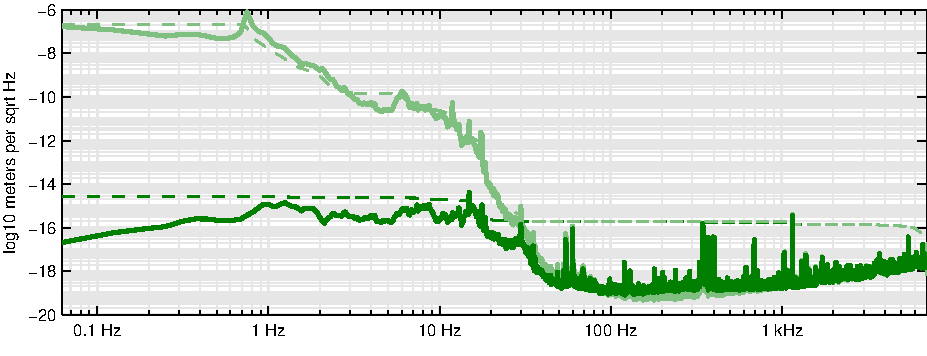
\includegraphics[width=\columnwidth]{figures/residualDARM.pdf}}
\caption[Residual DARM motion]{\label{fig:residual-DARM}Residual DARM}
\end{figure}

\subsection{Decrease in arm power due to off-resonance operation}

The decrease in buildup for a cavity operated off-resonance goes like
$(2\mathcal{F}/\pi)^2\phi^2$, where $\phi$ is the cavity detuning.
For $\mathcal{F}=220$ and $\phi=(2\pi/1064\text{ nm})(10\text{ pm})$,
the fractional power loss is only $7\times10^{-5}$.

\subsection{Decrease in power recycling gain due to power loss at the output port}
